\documentclass[12pt, a4paper]{report}
\usepackage[T1]{fontenc}
\usepackage[utf8]{inputenc}
\usepackage{bookman}
\usepackage{multicol}
\usepackage{tikz}
\usepackage{pgfplots}
\usepackage{german}
\usepackage{custompkg}
\usepackage[left=1.5cm,right=1.5cm,top=1.5cm,bottom=1.5cm]{geometry}
\usepackage{tabularx}
\pgfplotsset{compat=1.5}

\begin{document}
	\bslinespacing{1.5}
	\bsremovechaptertitle
	
	\chapter{Exponentialfunktionen}
	
	\section{Aufgabe 1}
	
		
	\begin{tabularx}{\textwidth}{|X|X|X|}
		\hline
		\textbf{Graph} & \textbf{Ableitungsgraph} &  \textbf{Funktion} \\
		\hline
		$G_1$ & $A_4$ & $f_1$ \\
		\hline
		$G_2$ & $A_3$ & $f_3$\\
		\hline
		$G_3$ & $A_2$ & $f_4$ \\
		\hline
		$G_4$ & $A_1$ & $f_2$ \\
		\hline
	\end{tabularx}
	
	\section{Aufgabe 2a}
	
	\begin{multicols}{2}
		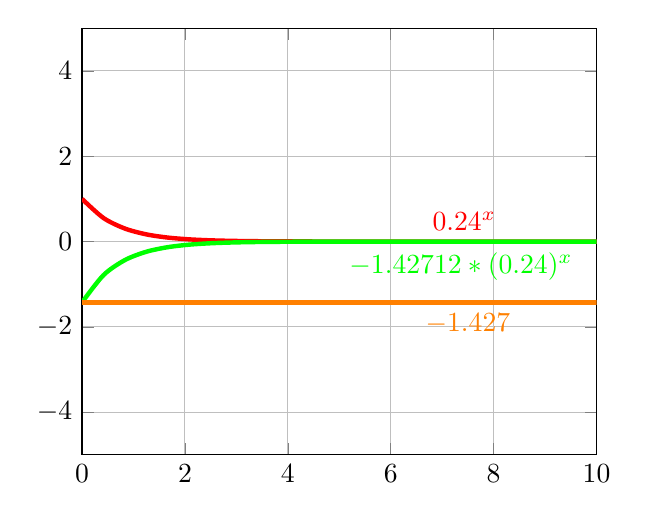
\begin{tikzpicture}[scale=1]
        	\begin{axis}
                [
                grid,
                xmin=0,
                xmax=10,
                ymin=-5,
                ymax=5,
                height=7cm
                ]

              \addplot[domain=0:10, color=red,smooth, ultra thick]{0.24^x} node[above,color=red,pos=0.75] {\color{red}$0.24^x$};
              \addplot[domain=0:10, color=green,smooth, ultra thick]{-1.42712*(0.24)^x} node[below,color=green,pos=0.75] {\color{green}$-1.42712*(0.24)^x $};
          	\addplot[domain=0:10, color=orange,smooth, ultra thick]{-1.427}  node[below,color=green,pos=0.75] {\color{orange}$-1.427$};
       	\end{axis}
    	\end{tikzpicture}
    	
    	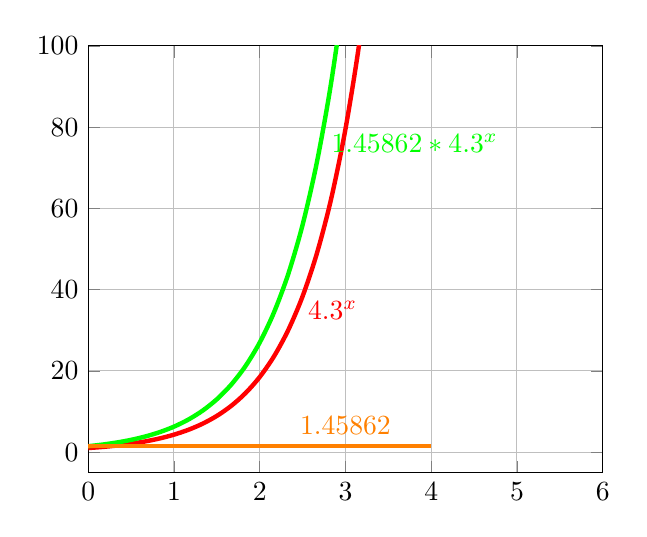
\begin{tikzpicture}[scale=1]
        	\begin{axis}
                [
                grid,
                xmin=0,
                xmax=6,
                ymin=-5,
                ymax=100,
                height=7cm
                ]

              \addplot[domain=0:4, color=red,smooth, ultra thick]{4.3^x} node[right,color=red,pos=0.10] {\color{red}$4.3^x$};
              \addplot[domain=0:4, color=green,smooth, ultra thick]{1.45862*4.3^x} node[right,color=green,pos=0.15] {\color{green}$1.45862*4.3^x$};
          	\addplot[domain=0:4, color=orange,smooth, ultra thick]{1.45862} node[above,color=green,pos=0.75] {\color{orange}$1.45862$};
       	\end{axis}
    	\end{tikzpicture}
	\end{multicols}

	\section{Aufgabe 2b}
	\Large$e=2.71828$\normalsize
	, geht durch die Berechnung mit dem GTR hervor.
	
	\newpage
	
	\section{Aufgabe 3a}
	\begin{enumerate}
		\item Für die Ableitung einer Exponentialfunktion vom Typ $f(x) = a^x (a>0)$ gilt also: $f'(x) = f'(0) \times a^x$
		\item $\frac{f(x+h) - f(x)}{h}$
		\item $=\frac{a^x \times a^h - a^x}{h}$
		\item $=\frac{a^{x+h} - a^x}{h}$
		\item $=\frac{a^x \times (a^h - 1)}{h}$
		\item $=a^x \times \frac{a^{0+h} - a^0}{h}$
		\item Die Ableitung einer Exponentialfunktion f ist somit proportional zu der Funktion f.
	\end{enumerate}
	
	\section{Aufgabe 3b}
	Laut Definition ist eine beliebige Zahl, die den Exponenten 0 hat, immer gleich 1.
	Dies gilt somit auch für die Eulersche-Zahl $e$
	
	\section{Aufgabe 3c}
	\paragraph{(1)}
	$f(1.000.000) = 2.71828$
	
	\paragraph{(2)}
	\begin{enumerate}
		\item $\frac{e^{0+h}-e^0}{h} \approx 1$
		\item Mit $h=\frac{1}{n}$ erhält man:
		\item $\frac{e^{\frac{1}{n}}-1}{\frac{1}{n}} \approx 1$
		\item $e^{\frac{1}{n}} - 1 \approx \frac{1}{n}$
		\item $e^{\frac{1}{n}} \approx 1 + \frac{1}{n}$
		\item $e = (e^{\frac{1}{n}})^n \approx (1 + \frac{1}{n})^n$
	\end{enumerate}
	


\end{document}